\documentclass[10pt,a4paper]{article}
\usepackage[utf8]{inputenc}
\usepackage[T1]{fontenc}
\usepackage[margin=0.55in]{geometry}
\usepackage[hidelinks,pdfnewwindow=true]{hyperref}
\usepackage{titlesec}
\usepackage{enumitem}
\usepackage{charter}
\usepackage{xcolor}
\usepackage{tikz}
\usetikzlibrary{shapes.geometric, arrows, positioning}

% Elegant, professional color palette
\definecolor{primary}{RGB}{30, 41, 59} % Deep Slate (Text & Headings)
\definecolor{accent}{RGB}{37, 99, 235} % Dynamic Blue for actionable items (links, subtle markers)
\definecolor{secondary}{RGB}{71, 85, 105} % Soft Slate for dates/locations
\definecolor{lightgray}{RGB}{241, 245, 249} % Very light slate for structure elements

\pagestyle{empty}

% Section formatting with clean accents
\titleformat{\section}
  {\normalfont\Large\bfseries\color{primary}\scshape}
  {}{0em}
  {}[\vspace{-2pt}\textcolor{accent}{\hrule height 1.5pt}]
\titlespacing{\section}{0pt}{14pt}{6pt}

\titleformat{\subsection}
  {\normalfont\large\bfseries\color{primary}}
  {}{0em}
  {}
\titlespacing{\subsection}{0pt}{8pt}{3pt}

% Highly dense, beautiful list spacing
\setlist[itemize]{leftmargin=*,noitemsep,topsep=1pt,parsep=1pt,partopsep=0pt}

% Job header macro for polished presentation
\newcommand{\jobheader}[4]{%
  \noindent%
  \textbf{\large #1} \hfill \textcolor{secondary}{\textbf{#2}} \\%
  \textit{\textcolor{accent}{#3}} \hfill \textit{\small\textcolor{secondary}{#4}}%
  \vspace{3pt}%
}

\begin{document}

% Header
\begin{center}
  {\Huge \textbf{\color{primary} JOHN OBA}} \\
  \vspace{4pt}
  {\large \textbf{\color{secondary} Software Engineer \ | \ Founding Engineer \ | \ Technical Lead}} \\
  \vspace{5pt}
  {\small 
    Nigeria \ | \ 
    \href{mailto:john.oba@afrodev.space}{\textcolor{accent}{john.oba@afrodev.space}} \ | \ 
    \href{https://linkedin.com}{\textcolor{accent}{LinkedIn}} \ | \ 
    \href{https://github.com}{\textcolor{accent}{GitHub}} \ | \ 
    \href{https://afrodev.space}{\textcolor{accent}{afrodev.space}}
  }
\end{center}

% Summary
\section{Professional Summary}
\noindent
\textbf{Pragmatic Software \& Product Engineer} with five years of experience building scalable, high-performance web applications across artificial intelligence, business intelligence, fintech, education, and real-time systems. Proven track record as a founding engineer and technical lead, translating ambiguous product visions into robust production systems. Expert in architecting modern frontends (React, Next.js, Vue) backed by resilient distributed services and database layers (NestJS, Laravel, FastAPI, PostgreSQL, Redis).

% Experience
\section{Professional Experience}

\jobheader{Oystack}{2025 -- Present}{Founding Engineer}{Remote}
\begin{itemize}
  \item \textbf{AI-Powered Research Platform:} Leading engineering for an AI research operating system designed for STEM researchers, focusing on connecting multi-modal sources, extracting key insights, and preserving document traceability.
  \item \textbf{Full-Stack Architecture:} Architected and delivered the initial MVP consisting of a NestJS backend, a responsive React/Tailwind CSS workspace dashboard, and a Plasmo-based browser extension for live web capturing.
  \item \textbf{Core Capabilities:} Built core features including page scanning, document parsing pipelines, seamless authentication, AI-generated context summaries, and reminder cron workflows.
  \item \textbf{Type-Safe AI Contracts:} Designed and enforced strict typed AI output schemas and validation workflows using Zod, ensuring zero-runtime failures from LLM-generated structured objects.
  \item \textbf{Product Strategy:} Partnered closely with the founder to rapidly translate initial concepts into technical requirements, user flows, and an actionable, high-velocity engineering roadmap.
  \item \textbf{Model-Agnostic Integration:} Integrated and abstracted multiple AI providers, maintaining clean separation between model-specific parameters and core business logic.
\end{itemize}

\jobheader{Startuplist Africa}{2021 -- Present}{CTO \& Co-founder}{Remote}
\begin{itemize}
  \item \textbf{Ecosystem Platform:} Co-founded and built Africa’s leading startup business intelligence platform, serving and engaging over \textbf{360,000 users}.
  \item \textbf{Engineering Leadership:} Own the end-to-end technical strategy, data architecture, deployment pipelines, performance optimization, and high availability of the platform.
  \item \textbf{Technology Stack:} Built the primary web services using Laravel, PostgreSQL, PGVector, Redis, and Vue.js with Quasar for server-side rendering (SSR) and optimal SEO performance.
  \item \textbf{Data \& Intelligence Products:} Engineered interactive startup comparison matrices, funding deal trackers, pitch-deck evaluators, and automatic data ingestion routines.
  \item \textbf{Semantic Search:} Integrated vector embeddings and PGVector-powered similarity search to dramatically improve startup, investor, and market report discovery.
  \item \textbf{Infrastructure \& DevOps:} Managed and optimized high-performance deployments across Vercel, Heroku, Cloudflare, and GitHub Actions CI/CD.
\end{itemize}

\jobheader{KP Astro}{Feb 2025 -- Aug 2025}{Founding Engineer}{Remote}
\begin{itemize}
  \item \textbf{Niche SaaS Launch:} Served as the sole founding engineer, building and launching a specialized astrology platform actively used by \textbf{over 2,000 verified astrologers}.
  \item \textbf{Domain Modeling:} Mastered complex mathematical and astrological rules of KP Astrology, converting planetary calculations, birth charts, South Indian charts, transits, and almanac datasets into performant algorithms.
  \item \textbf{Distributed Architecture:} Designed and operated a robust distributed backend using Django, FastAPI, Apache Kafka, Redis, and PostgreSQL with containerized workers.
  \item \textbf{Core Features:} Developed reusable prediction templates, automated PDF/CSV report generation, and real-time chart updating services.
  \item \textbf{Engagement Metrics:} Achieved an exceptional average session duration of \textbf{49 minutes} due to ultra-fast background processing, custom caching layers, and responsive UI design.
\end{itemize}

\jobheader{Niyo Group / Niyo Labs}{Nov 2023 -- Oct 2024}{Frontend Developer to Technical Lead}{Hybrid}
\begin{itemize}
  \item \textbf{Rapid Promotion:} Promoted from Frontend Developer to Technical Lead, taking charge of architecture, code quality, and delivery of an online collaborative learning platform.
  \item \textbf{Real-Time Features:} Built the signature ``Learn with Friends'' experience using Socket.io, NestJS Gateways, and Agora RTC for low-latency voice and video integration.
  \item \textbf{Interactive Workspace:} Implemented synchronized video playback, real-time participant presence, host controls, and dynamic speaking indicators.
  \item \textbf{Core Auth \& Onboarding:} Delivered passwordless authentication, streamlined onboarding funnels, custom quizzes, and on-demand PDF certificate generation.
\end{itemize}

\jobheader{Nomba}{Feb 2023 -- Nov 2023}{Frontend Engineer}{Lagos, Nigeria}
\begin{itemize}
  \item \textbf{Fintech Interfaces:} Designed and built high-performance marketing and product frontends for Nomba's flagship merchant tools (Nomba Max, Mini, Invoice, Menu, and Terminal) using React, Gatsby, and Tailwind CSS.
  \item \textbf{Cinematic Interactions:} Created highly polished, fluid interactive experiences and landing pages using GSAP (GreenSock) and ScrollTrigger.
\end{itemize}

\jobheader{Nigeria Police Force, Supernumerary Unit}{Feb 2022 -- Jan 2023}{Frontend Engineer}{Nigeria}
\begin{itemize}
  \item \textbf{Digital Initiatives:} Developed responsive web portals and frontend interfaces for internal operational systems and public-facing digital initiatives, collaborating closely with key security stakeholders.
\end{itemize}

\jobheader{AfroLabs}{Aug 2021 -- Dec 2021}{Software Engineer}{Remote}
\begin{itemize}
  \item \textbf{Web3 \& Automation:} Built decentralized finance integrations, automated Discord bots, and wallet-connected tools using EIP-3009 (USDC gasless transactions) and real-time blockchain event listeners via Alchemy WebSockets.
\end{itemize}

% Projects
\section{Selected Projects}
\begin{itemize}
  \item \textbf{Box.tools}: Created a comprehensive utility suite of over 45 high-performance browser-based tools for developers and business users, serving local data transformations instantly.
  \item \textbf{PeerPlay}: Developed an open-source real-time synchronized media playback and chat engine using Next.js and Socket.io.
\end{itemize}

% Technical Stack Diagram
\section{Technical Skills \& Architecture Stack}
\noindent
\begin{minipage}[t]{0.45\textwidth}
\vspace{0pt}
\begin{itemize}[label=\raisebox{0.25ex}{\tiny$\bullet$}]
  \item \textbf{Languages:} TypeScript, JavaScript, Python, PHP, SQL, HTML, CSS
  \item \textbf{Frontend Frameworks:} React, Next.js, Vue.js, Nuxt, Quasar, Tailwind CSS
  \item \textbf{Backend \& Real-Time:} NestJS, Node.js, Laravel, Django, FastAPI, WebSockets
  \item \textbf{Databases \& Cloud:} PostgreSQL, PGVector, Redis, Docker, AWS, GitHub Actions
  \item \textbf{AI Engineering:} LLM Structured Outputs, Prompt Engineering, RAG
\end{itemize}
\end{minipage}
\hfill
\begin{minipage}[t]{0.50\textwidth}
\vspace{-15pt}
\begin{center}
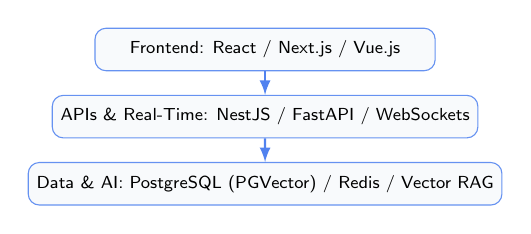
\begin{tikzpicture}[
  scale=0.9, every node/.style={scale=0.9},
  box/.style={rectangle, draw=accent!70, fill=lightgray!50, rounded corners=4pt, minimum width=4.8cm, minimum height=0.6cm, align=center, font=\bfseries\sffamily\scriptsize},
  arrow/.style={-latex, thick, accent!80}
]
  % Nodes
  \node[box] (fe) {Frontend: React / Next.js / Vue.js};
  \node[box, below=0.3cm of fe] (api) {APIs \& Real-Time: NestJS / FastAPI / WebSockets};
  \node[box, below=0.3cm of api] (db) {Data \& AI: PostgreSQL (PGVector) / Redis / Vector RAG};

  % Paths
  \draw[arrow] (fe) -- (api);
  \draw[arrow] (api) -- (db);
\end{tikzpicture}
\end{center}
\end{minipage}

\vspace{10pt}

% Education
\section{Education}
\noindent
\textbf{University of Nigeria, Nsukka} \hfill Nsukka, Nigeria \\
\textit{Bachelor of Science in Pure and Industrial Chemistry} \hfill \textit{Class of 2021} \\
\textbf{CGPA: 4.21 / 5.00}

\end{document}
